\hypertarget{working-environment}{%
\chapter{Working Environment}\label{working-environment}}
This chapter explains the technical environment for the laboratory. This
includes the usage of the computers and the directory structure for this
laboratory. It is very important to understand completely the directory
structure, as many scripts rely on this special structure and will not
work at all or create an unexpected output if the directory structure is
set up in a wrong way.
\hypertarget{network-structure}{%
\section{Network Structure}\label{network-structure}}
The programs needed to perform the laboratory tasks run under Linux. You
will work with the computers in the lab 308.2. This room has 10
computers with Ubuntu 14.04, 32bit installed and are named as follow:
\begin{lstlisting}
i83labpcXX.itec.kit.edu where XX=01, 02, \ldots{} 10.
\end{lstlisting}
These computers can also be accessed remotely via SSH or via X2Go
Client, see \protect\hyperlink{remote-operation}{Chapter 2.2.1} and
\protect\hyperlink{x2go-client}{2.2.2}. The user name like asipXX where
XX=01, 02\ldots, 10 and password to login to these computers for
different student groups will be distributed at the beginning of the
lab. You can also access these computers from student lab (Room 312.4)
or from your personal Laptop. X2Go Client is already installed on all
computers in the student lab (Room 312.4) while you have to install and
configure X2Go Client on your Laptop at your own. It is recommended to
use SSH instead of X2Go as it has some conflicts with some settings.

For ASIPmeister and GCC compiler, it is necessary to change the machine
in order to meet the software requirements. There is one dedicated
application workstations:
\begin{lstlisting}
i83pc57.itec.kit.edu -- ASIPmeister system:
\end{lstlisting}
You will use this PC for building your own customized CPU and compiler
that is able to use the instructions you added to the instruction set of
the basic processor. This task also needs a powerful machine to complete
in a reasonable amount of time.

To run, this lab, you need to export the following variables, or you can
add it the your /home/.bashrc.user.
\begin{lstlisting}
export ASIPS_LICENSE=29000@i83asip.itec.kit.edu
export PATH=/AM/ASIPmeister/bin:$PATH
export ASIP_APDEV_SRCROOT=~/AM_tools
export PATH=/usr/java/jre1.6.0_45/bin:$PATH
export ASIPmeister_Home=/AM/ASIPmeister
export ASIPmeister_HOME=/AM/ASIPmeister
source /home/adm/modelsim_66d.setup
source /home/adm/xilinx_13.2_32bit.setup
\end{lstlisting}
In most cases, you have to manually login into this machine to work with
the ASIPmeister and GCC Compiler. We will provide you the scripts that
will do most of the work for you. Just be aware of the fact that it will
sometimes take time to complete everything. If some errors occur, try to
find out what is wrong by reading the script output carefully. This will
show what went wrong. Start again and if it fails again then ask your
tutor. The most important thing is to know or to recognize that the
results of the script task are right or wrong. This depends on the
output, so read it carefully before starting the next task.

The lab program directory is mounted via NFS to your client. Thus,
almost every program will work on your local machine. Data supplied to
the groups or created by them will be stored on a server directory that
is always available for a client machine. All client machines are
configured as NFS clients, which mount the corresponding home directory
via NFS. This means you can work wherever you want. The hostname will
change, but your home directory will show the same content on all
clients.

To switch between the machines mentioned above you have to use SSH
(recommended). The names of the client PCs are similar to
i83labpcXX.itec.kit.edu with the `XX' replaced by the individual number of
the PC. Login with SSH requires authentication, which can be done with
passwords or public keys (see
\protect\hyperlink{remote-operation}{Chapter 2.2.1}). In order to
minimize the efforts for changing machines we recommend public keys, so
you do not have to type your password for every remote login.

\hypertarget{basic-unix-commandsprograms}{%
\section{Basic UNIX
Commands/Programs}\label{basic-unix-commandsprograms}}

If you are familiar with the Unix/Linux environment, you can skip this
section. In this section, ``Unix'' will refer to GNU/Linux mostly.

\begin{itemize}
\item
  \textbf{Command Line Interpreter}: Interaction with the system usually
  is done via the command line, although some file system operation can
  be done with graphical or text based file managers.

The command line interpreter (generally called ``shell'') runs on a
terminal and primarily provides the user with the means to start
programs. It also has several built in commands as well as a scripting
language. The default shell in the lab is \emph{bash} (Bourne Again
Shell).

Some programs and commands require command line arguments (parameters),
which can be supplied in a space-separated list to the program, i.e.:

\emph{cp file1 file2} executes the program ``\emph{cp}'' with the
arguments ``\emph{file1}'' and ``\emph{file2}''.

\item
  \textbf{Online Help System}: Most UNIX commands come with
  documentation in the manual page format (\emph{man}-pages). They
  usually give a detailed description of the program, all command line
  parameters, and some examples. Use the \emph{man} command to read
  \emph{man}-pages, i.e.: ``\emph{man ls}'' calls the \emph{man}-page
  for the ``\emph{ls}'' command. Use the up and down arrow keys (or Page
  Up/Down) to navigate in the man page viewer and ``\emph{q}'' to quit.
\item
  \textbf{Interacting with the File System}
  \begin{enumerate}
  \item
    \textbf{File System Structure}: UNIX organizes all files (regular
    and special files) in a tree structure. The root of the tree is
    called ``/'', directories are the nodes (leaf or non-leaf) and files
    the leaf nodes of the tree. The file system does not have a concept
    of drives -- new data from external media (networked or removable)
    is accessed by attaching the sub tree of the new file system to the
    UNIX file system tree somewhere. Usually ordinary users are not
    permitted to do this.
  \item
    \textbf{Working Directory}: Every process has a current working
    directory -- a pointer to a directory node in the file system tree.
    The current working directory is referred to as ``.'' and the parent
    directory as ``..''. To print the current working directory of the
    shell, use the command ``\emph{pwd}'' (print working directory).
  \item
    \textbf{Home Directory}: Every user has a home directory -- one for
    which he has write access. All your data will be saved in
    subdirectories of your home directory. Home directories are mounted
    via NFS from a remote server. Home directories have the form of
    ``\emph{/home/asip01''} but a user can refer to his home directory
    with ``\emph{\textasciitilde{}}''. Hence,
    ``\emph{/home/asip01/test}'' and ``\emph{\textasciitilde/test''}
    (executed by the user ``\emph{asip01}'') refer to the same.
  \item
    \textbf{File Paths}: To specify a file or a directory, a path name
    must be provided. There are two kinds of paths: absolute and
    relative. An absolute path starts at the root directory, a relative
    path starts at the current working directory. File system nodes
    (path name components) are separated by ``/'' (the same as the
    backslash in Windows). A relative path may be like
    ``\emph{./ASIPMeisterProjects/browstd32}'' which refers to the file
    or directory ``\emph{browstd32}'' of the subdirectory
    ASIPMeisterProjects of the current working directory. An example for
    an absolute path for the same relative path is
    ``\emph{/home/asip01/ASIPMeisterProjects/browstd32}''.
  \item
    \textbf{Changing the Current Working Directory}: To change the
    current working directory use the \emph{cd} command with a path name
    as the argument, i.e.:
\begin{lstlisting}
cd /home/asip01
cd ..
cd ../asip02/ASIPMeisterProjects
cd ./browstd32/Applications
\end{lstlisting}
\item
  \textbf{Creating/Removing Directories}: the ``\emph{mkdir}'' command
  takes a pathname as an argument and creates a new directory accessible
  via this path. The ``\emph{-p}'' parameter tells mkdir to create any
  missing subdirectories as well. ``\emph{rmdir}'' deletes empty
  directories. To remove non-empty directories use the ``\emph{rm}''
  command with the ``\emph{‑r}'' option (see below). Some of the
  examples are:
\begin{lstlisting}
mkdir ~/ASIPMeisterProjects/browstd32/Applications
rmdir ../browstd32/test1
mkdir -p ~/some/non_existing/directory
\end{lstlisting}
\item
  \textbf{Listing Directory Contents}: To examine directory contents use
  the ``\emph{ls}'' command. Without parameters, it will show the file
  and directory names of the current working directory. The
  ``\emph{ls}'' command has many parameters, all described in the
  man-page. Typical ones are ``\emph{‑l}'' to provide a detailed
  listing, ``\emph{‑a}'' to show hidden files (filenames starting with a
  ``.''), ``\emph{‑ltc}'' gives a detailed listing with the last file
  modification time and sort by it (actually these are three
  parameters). Some of the examples are:
\begin{lstlisting}
ls
ls -l ../ASIPMeisterProjects
ls -ltc ASIPMeisterProjects/browstd32/ModelSim
\end{lstlisting}
\item
  \textbf{Moving and Removing Files}: To move or rename a file use the
  ``\emph{mv}'' command with the filename or directory as the argument.
  To remove a file use ``\emph{rm''}; the ``\emph{‑r}'' option causes
  recursive removal of subdirectories and their contents. Some of the
  examples are:
\begin{lstlisting}
mv Applications/tset Applications/test
rm /home/asip01/oldfile
rm -r ../browstd32
\end{lstlisting}
\item
  \textbf{Copying Files}: The ``\emph{cp}'' command copies files and
  directories. Its arguments are: optional switches, then the source and
  the target file/directory respectively. The ``\emph{‑r}'' switch
  enables recursive copying. Some of the examples are:
\begin{lstlisting}
cp TestData.IM TestData.IM-backup
cp -r browstd32 browstd32\_custom
\end{lstlisting}
\end{enumerate}
\item \textbf{Shell Operation:}

  \begin{enumerate}
  \item
    \textbf{Input/Output Redirection}: Some programs read data on their
    standard input file descriptor (stdin), some write output to the
    standard output (stdout). Usually stdin is linked to the keyboard
    and stdout to the terminal screen. However, you can change this when
    calling a program. ``\emph{\textless{} somefile}'' redirects stdin
    to read from ``\emph{somefile}'' and not from keyboard, likewise
    \emph{``\textgreater{} someotherfile}'' will redirect stdout to
    write to ``\emph{someotherfile}'' (if it doesn't exist, it will be
    created, if it does, it will be truncated first -- use
    ``\emph{\textgreater\textgreater{} someotherfile}'' to append
    instead of truncating the previous contents. Redirection is also
    possible to/from other processes via pipes: use ``\emph{program1
    \textbar{} program2}'' to direct the output of ``\emph{program1}''
    to the input of ``\emph{program2}''. Some of the examples are:
\begin{lstlisting}
ls -ltc >filelisting
ls | sort
cat <file1 >>file2 (this appends the contents of file1 to file2).
\end{lstlisting}
\item \textbf{Job Control}: Processes started from the shell are often
  referred to as ``\emph{jobs}''. Usually, when the shell launches a
  program it will take control of the terminal and the shell will be
  suspended until the process terminates -- the job ``is running in the
  foreground''. To launch a job ``in the background'' -- start it, but
  give control back to the shell immediately, append ``\&'' at the end
  of parameter list. To list any jobs launched from this shell (they all
  have to be in the background), type ``\emph{jobs}'' -- this will give
  you the job-IDs with the program names and parameters of the jobs. To
  bring a job to the foreground, use ``\emph{fg \%job-ID}'' (substitute
  job-ID for the actual job ID). Sometimes you will want to temporarily
  stop a job -- if the program is in the foreground, hit ``CTRL-Z'' (job
  suspension). To continue job execution in the foreground use
  ``\emph{fg}'' as described above, or ``\emph{bg \%job-ID}'' to
  continue execution in the background.
\end{enumerate}

To terminate a job in the foreground, hit ``CTRL-C'' (send keyboard
interrupt). Note that if a process is unresponsive (due to bugs -- i.e.
endless loop and signal processing disabled) it can ignore this; the
only way to terminate it is to send a KILL signal as explained below).
\item
  Some important programs and commands
  \begin{enumerate}
  \item
    \textbf{Process/Activity Listing}. To view a complete list of
    running processes, use the ``\emph{ps}'' program. It is mostly used
    with the ``\emph{auxw}'' options to provide a complete and detailed
    listing. The output is usually quite long, so it is often piped into
    ``\emph{less}'' or ``\emph{head}''.
  \item
    \textbf{Text Viewer}. ``\emph{less}'' is a program to view text (you
    can use it to view binary data as well, but it treats it as a byte
    stream without any special formatting, except for control characters
    -- they are substituted). The argument is the file to view;
    otherwise, data can be piped if used without any arguments. To
    scroll through the ``\emph{less}'' output use the up and down arrow
    keys (or Page Up/Down) to navigate, ``\emph{q}'' to quit. To jump to
    a specific line (current line and byte numbers are displayed at the
    bottom), type the line number followed by \emph{G} (i.e. \emph{123G}
    to jump to line 123). Some of the examples are:
\begin{lstlisting}
less ModelSim/TestData.DM
ps axuw | less
\end{lstlisting}
\item
  \textbf{Difference between Files}: The ``\emph{diff}'' program
  examines two files for differences and displays these. Useful to
  compare outputs of programs and see if and what changes occurred.
  Common options are ``\emph{‑u}'' (unified output) to have verbose
  output. Unified output lists the lines that were in the old file, but
  are not in the new file preceded with a ``-`` and files that were not
  in the old file and are in the new file preceded with a ``+''. Lines
  that start with neither are just context to make orientation a bit
  easier. File sections where changes were detected start with @@,
  followed by the line ranges of the sections. A graphical diff-tool
  that visualizes the output of ``\emph{diff}'' is ``\emph{kompare}''
  (the `k' instead of `c' for `compare' denotes that it is meant for
  kde; so this is not a typing error). Some of the examples are:
\begin{lstlisting}
diff -u TestData.DM-OLD TestData.DM | less
kompare EvilFile.txt GoodFile.txt &
\end{lstlisting}
\item
  \textbf{Show only the Beginning/End of a File/Output}. The
  ``\emph{head}'' and ``\emph{tail}'' programs show only the first and
  last lines (respectively) of a file or the data that are piped in. By
  default they show 10 lines, but the ``\emph{‑n x}'' option sets it to
  x lines. Tail can also monitor a file for future appends and display
  them (useful when watching log files of a running program). This is
  requested with the ``\emph{‑f}'' option. Some of the examples are:
\begin{lstlisting}
ls -ltc Applications/bubblesort | head -n 5
tail -n 0 -f /tmp/logfile
\end{lstlisting}
\item
  \textbf{Show Machine's Activity Summary}: while the ``\emph{ps}''
  command gives a detailed overview of the running processes, sometimes
  a summary is more useful. ``\emph{top}'' shows the current number of
  running processes, the CPU(s), memory and swap usage and the active
  processes. It updates every three seconds and can be exited with
  ``\emph{q}''.
\end{enumerate}
\end{itemize}
\hypertarget{remote-operation}{%
\subsection{Remote Operation}\label{remote-operation}}
\begin{enumerate}
\item
  \textbf{Remote login}. To log onto a different machine, the SSH
  program is available (Secure Shell). Communication between the two
  machines is encrypted by SSH. To simply log onto a different machine
  with the current user, use ``\emph{ssh~hostname}''. If your account
  username is not the same as on the local machine use
  ``\emph{ssh~otheruser@hostname}'', where ``\emph{otheruser}'' is the
  username of the account on the remote machine. SSH will ask for a
  password on the remote machine, and then log in and start a shell.
  ``\emph{exit}'' will end the remote shell and terminate the SSH
  connection leaving you on your local machine.
\item
  \textbf{Copying via SSH}: Not all machines have NFS mounted home
  directories, so you will sometimes have to copy files to a remote
  machine. The SSH package provides ``\emph{scp}'' for this, which can
  copy files or directories from one machine to another (if you have an
  account on the remote machine). The syntax is ``\emph{scp somefile
  remotehost:}'' (note the colon at the end, omitting it will cause scp
  to copy ``somefile'' to the file ``remotehost'' on the local machine).
  To copy directory trees use ``\emph{scp -r directory remotehost:}''
\item
  \textbf{X11 Forwarding}: GUI programs can be run on remote machines as
  well. Log in on a remote machine with ``\emph{ssh -X remotehost}'' and
  start a program installed on remotehost. It will be displayed on your
  machine, but will run (access files and use resources -- CPU, memory,
  etc.) on remotehost.
\item
  \textbf{Public Key Authentication}. An alternative to providing
  passwords for every login is public key authentication mode. A key
  pair is created on your local machine and you can copy the public key
  to any machine you want to log on later. Once set up, authentication
  is done automatically and no interactive passwords are necessary. The
  steps to setup a public key authentication is as follows:

  \begin{enumerate}
  \def\labelenumii{\roman{enumii}.}
  \item
    First, create the DSA-keys by logging into any machine and invoking:
\begin{lstlisting}
ssh-keygen --t dsa
\end{lstlisting}
Confirm the default destination for the keys. Afterwards enter your pass
phrase, for example, your group name or you can just leave it empty.
Sometimes you will be asked for this, so remember what you entered.
Public and private keys will be stored in your
``\emph{\textasciitilde/.ssh}'' directory.
\item
  Then copy the public key to the remote machine:
\begin{lstlisting}
ssh-copy-id --i \textasciitilde/.ssh/id\_dsa.pub user@remote-machine
\end{lstlisting}
\end{enumerate}
\end{enumerate}
Enter your password to confirm this step. Afterwards log out and try to
log in again. This should work without asking you to enter the password.

\hypertarget{x2go-client}{%
\subsection{X2Go Client}\label{x2go-client}}

X2Go is a program used to run graphical applications on Linux machines
remotely. This uses a technology, which results in better performance.
This also allows for suspending and resuming sessions and programs,
while they are running. This allows the use of long-running graphical
applications.

\begin{itemize}
\item
  Installation
  \begin{enumerate}
  \def\labelenumi{\alph{enumi}.}
  \item
    The X2Go Client software is already installed on all computers in
    out student lab.
  \item
    For your Laptop, you can download and install the X2Go Client from:
    \url{http://wiki.x2go.org/doku.php/download:start}
  \end{enumerate}
\item
  Configuration

When you first run the X2Go client, a "\emph{New session}" dialog should
appear otherwise you can create new session using ``\emph{Session}''
menu and then clicking on ``\emph{New Session\ldots{}}'' You should fill
this in with the following information in ``\emph{Session}'' tab:
\begin{enumerate}
\def\labelenumi{\alph{enumi}.}
\item
  Session name - Any name you like to identify the session - if you're
  connecting to the PC ``\emph{i83labpc01}'', you might just want this
  to be " \emph{i83labpc01}"
\item
  Host - Full name of the computer you're connecting to, e.g.
  ``\emph{i83labpc01.itec.kit.edu}''
\item
  Login - Your user ID, for example ``\emph{asip01}''
\item
  Session type - Select XFCE (recommended) - This is a low-power window
  manager that is the only one supported in the current version of
  Ubuntu.
\item
  Keep all the other setting to default.
\end{enumerate}
\item
  Connecting
  \begin{enumerate}
  \def\labelenumi{\alph{enumi}.}
  \item
    To start the session, click on it and enter your password when
    prompted
  \item
    After you click OK, it will connect to the server and start your
    session. Watch the Status line to see what is happening. Once the
    status is "running," your session should launch.
  \item
    Sometimes "\emph{i83labpcXX}" cannot be accessed remotely using
    X2Go, while it works fine with SSH. May be there is a conflict
    between some settings in your \textasciitilde/.bashrc.user and X2Go.
    For example one temporary solution is to comment out the line ".
    /home/adm/xilinx\_13.2\_32bit.setup" in
    \textasciitilde/.bashrc.user. This makes X2Go work properly. If
    Xilinx ISE is required, you can source it manually.
  \end{enumerate}
\end{itemize}
\hypertarget{directory-structure}{%
\section{Directory Structure}\label{directory-structure}}
In development environments it is very useful to force developers to
meet certain rules how program data is stored. Therefore, we provide a
template that makes it easier for the tutors to find the results of
every group and enables us to write script files that work on fixed
locations to speed up the work. On the other hand, these script depend
on this directory structure. You have to understand and use this
directory structure to avoid problems.

The main directory structure is shown in Figure \ref{fig:fig21}. Your home directory contains one
special directory called ``\emph{ASIPMeisterProjects}''. All your
ASIPMeister Projects including your applications and all other files
will be placed in this directory. Inside this
``\emph{ASIPMeisterProjects}''-directory every project has a
subdirectory (e.g. ``\emph{browstd32}'' or ``\emph{AnotherProject}'').
We recommended that you create new subdirectory/project for each changed
version of the CPU. Among the projects the
``\emph{ASIPMeisterProjects}''-directory also includes a
``\emph{TEMPLATE\_PROJECT}''. This directory gives you a basic ASIP
Meister Project with minimum director structure and files required to
start your ASIP projects. This template is a good starting point to
create a new project from the scratch. Usually you can copy from your
last project to create a new one, but sometimes it is recommended to
start from the scratch.
\begin{figure}[!htb]
	\centering
	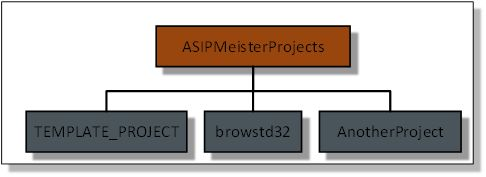
\includegraphics[width=0.9\textwidth]{src/images/2-1.png}
	\caption{ The Directory Structure for all ASIP Meister Projects}
	\label{fig:fig21}
\end{figure}
The biggest part of the directory structure is placed inside each ASIP
Meister project directory, e.g. ``\emph{browstd32}'', as shown in Figure
\ref{fig:fig21}. Every project directory contains
\textbf{five} subdirectories and a set of local files. These directories
and files are explained in the following sections.

The \textbf{``Applications''} directory should contain all your user
applications that you want to run and simulate on the CPU, each in a
separate subdirectory. Every application should be placed inside a
separate subdirectory for this application along with a \emph{Makefile}
that is needed to compile, simulate and implement the application. When
you want to compile an application, simulate it (dlxsim or ModelSim),
generate its bitstream for FPGA, or upload its bitstream into FPGA, you
run the \emph{Makefile} in that particular application subdirectory. To
see different options that \emph{Makefile} offers, execute
``\emph{\textbf{make}}'' in an application subdirectory, as shown below:
\begin{lstlisting}
asip04@i83labpc04:~/ASIPMeisterProjects/browstd32/Applications/Application1:$make
/--------
| USAGE:
\--------
'make sim':    compile for dlxsim/Modelsim
'make dlxsim': compile for dlxsim and directly start simulation
'make fpga':   compile for FPGA and update bitstream
'make upload': upload the existing bitstream to the FPGA (note: this command does not generate a new bitstream)
'make all':    compile for dlxsim/Modelsim and for FPGA
'make clean':  delete the BUILD directories

/---------------------
| PASSING PARAMETERS:
\---------------------
'DLXSIM_PARAM=...'
Example: 'make dlxsim DLXSIM_PARAM="-da0 -pf1"'
Note:    These are the default parameters. Don't forget the double high-commas (i.e.: ") when passing multiple parameters.
'GCC_PARAM =...'
Example: 'make sim GCC_PARAM =-O3'
Example: 'make dlxsim GCC_PARAM =-O3 DLXSIM_PARAM="-da0 -pf1"'
Note:    If you want to enfore re-compilation with different parame-ters then you have to 'make clean' to make sure that all files are re-compiled
\end{lstlisting}
For example, if you want to work with ``\emph{Application1}'', as shown
in Figure \ref{fig:fig23}. Your first step is to compile
this application. Inside the ``\emph{Application1}'' directory
containing source code ``\emph{application1.c}'' or
``\emph{application1.s}''. To compile it you have to execute the
following in the ``\emph{Application 1}'' directory:

asip04@i83labpc04:\textasciitilde/ASIPMeisterProjects/browstd32/Applications/Application1:\$make
sim

The \emph{Makefile} is expected to be executed from the directory, where
the results will be placed, so always execute the scripts from the
application specific subdirectory, never from the
``\emph{Applications}'' directory itself! The details about the
parameters, the created output files and the different versions of the
Makefile scripts are explained in Table \ref{fig:fig22}.
The concept of calling the scripts from the specific application
subdirectory is also important for the Makefile script while executing
``\emph{make sim}'', ``\emph{make dlxsim}'', ``\emph{make fpga}'' and
``\emph{make upload}'' as explained in Table \ref{fig:fig22}.
\begin{table}[!htb]
	\centering
	\begin{tabular}{|l|p{13cm}|}
		\hline
		\multicolumn{1}{|c|}{\textbf{Script}} & \textbf{Description}                                                               \\ \hline
		make sim 
		& It will compile your assembly or C-file file in your current application
		directory and ``\emph{BUILD\_SIM}'' subdirectory is created in your
		current directory containing different files like ``\emph{TestData.IM}''
		and ``\emph{TestData.DM}'' file for the ModelSim. The output assembly
		file named ``NameOfTheApplication-Directory.dlxsim'' will also be
		generated. You can pass different parameters to this Makefile as
		follows:
		\begin{enumerate}
			\item
			\emph{GCC\_PARAM} is used to set optimization level for GCC Compiler.
			The compiler options are directly forwarded to the compiler binary
			e.g. ``-O0'' or ``-O4'' for different optimization levels. for
			example:
		\end{enumerate}
		make sim GCC\_PARAM =-O3\strut \\\hline
		make dlxsim      
		& It will start the dlx simulator to simulate the compiled file generated
		from the previous stage. Similar to previous command,
		``\emph{BUILD\_SIM}'' containing different files like
		``\emph{TestData.IM}'', ``\emph{TestData.DM}'' and
		``NameOfTheApplication-Directory.dlxsim'' is created. Here, you have to
		pass some parameters to dlxsim mentioned in the Figure. You can also
		pass \emph{GCC\_PARAM} with this command. Another parameter that is
		required with this command is DLXSIM\_PARAM, which is used to pass
		different dlxsim parameters, for example:
		
		make dlxsim DLXSIM\_PARAM="-fAppName.s -da0 --pf1 -lfputc.out "
		
		In the command, ``\emph{AppName.s}'' is loaded into dlxsim for
		simulation, without debugging and with pipeline forwarding. Moreover,
		``\emph{putc.out}'' is the file containing the printed output. Executing
		``\emph{make dlxsim}'' without any parameters, will execute the file
		``\emph{BUILD\_SIM/AppName.dlxsim}'' with ``\emph{-da0}'' and
		``\emph{-pf1}''.\strut  \\\hline
		make dlxsim-test        
		& To disrupt, emancipate, transform the habitus and field of design To explore how the user is affected by design practices, objects and systems To change design practices, \\\hline
		make fpga &       
		It will compile your assembly or C-file, generate the
		required DM/IM file, and combine them with your bitstream that is
		generated from the ISE Project. Finally, a new bitstream file containing
		your hardware CPU along with corresponding IM/DM files of your
		application will be generated in the subdirectory ``\emph{BUILD\_SIM}''.
		This bitstream will be used to configure the FPGA. \\ \hline
		make upload &        
		It will upload the existing bitstream to the FPGA
		BlockRAM. Note that this command does not generate a new
		bitstream. \\ \hline
		make clean &       
		It cleans your current project directory by deleting
		``\emph{BUILD\_SIM}''. \\	\hline
		make all &       
		It will compile for dlxsim and for ModelSim and generate
		final bitstream for FPGA. \\	\hline
	\end{tabular}
	\caption{Makefile Options and Parameters}
\label{fig:fig22}
\end{table}
\begin{figure}[!htb]
	\centering
	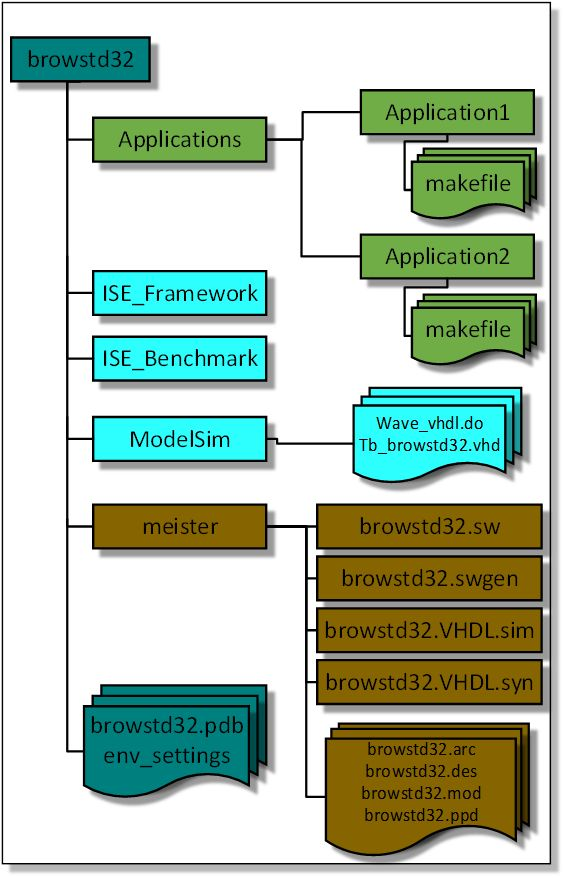
\includegraphics[width=0.8\textwidth]{src/images/2-3.png}
	\caption{The Directory Structure for a Specific ASIP Meister Project}
	\label{fig:fig23}
\end{figure}
The \emph{Makefile} script inside the ``\emph{Applications}'' directory
is only wrapper for the real scripts. This wrapper first read the
``\emph{env\_settings}'' file from your project directory (e.g.
``\emph{browstd32}'' in Figure \ref{fig:fig23}). This
file contains all the information about your current project, e.g. which
compiler to use and which dlxsim to call. Afterwards the wrapper script
calls the real scripts. The real scripts are placed at a global
position. This enables us to make changes to these scripts without the
need to copy these changes to all your projects. The
``\emph{env\_settings}'' file is explained in Table \ref{fig:fig25}.

The \textbf{``\emph{meister}''} directory contains the ASIP Meister
output, like the VHDL and compiler generation files. ASIP Meister
automatically creates this ``\emph{meister}'' directory. This meister
directory is always created at the place, where ASIP Meister is started.
So execute ASIP Meister inside your project directory (\emph{browstd32}
in this example)! It is very important, that you always start ASIP
Meister in your current project directory. Otherwise, the other scripts
will not find the meister subdirectory or even worse: they work with an
old version of the meister directory. The directory ``\emph{meister}''
contains three subdirectories for the simulation VHDL files
(\emph{browstd32.sim}), the synthesis VHDL files (\emph{browstd32.syn})
and the software description (\emph{browstd32.sw}) respectively for the
project ``\emph{browstd32}''. Some additional files are placed inside
the meister directory itself. The most important file here is the
``\emph{browstd32.des}'' file. This file contains all information that
is required to create a binary file out of an assembly file, i.e. to
assemble an assembly file. This file can be automatically extended with
user instructions, as explained in Figure 2‑4:. From the subdirectories,
you will mostly need the VHDL files from ``\emph{browstd32.syn}'' for
simulation in ModelSim as explained in Chapter~5 and for synthesis as
explained in Chapter~6. Inside the ``\emph{browstd32.sw}'' directory,
which is needed for creating the GCC compiler, you will mostly need the
``\emph{instruction\_set.arch}'' file, as explained in Chapter~8.2. This
file contains the summary of all assembly instructions that the compiler
will support, but sometimes this file has to be manually edited before
starting the automatic compiler generation.

The \textbf{``ModelSim''} directory will contain your ModelSim project
for simulating the CPU at VHDL level. ModelSim itself is explained in
Chapter~5. It is important, that you start ModelSim inside this
``\emph{ModelSim}'' directory, as it searches for specific files at the
position where it was started. There are \textbf{five} files already
placed in this directory containing the test bench and some
configuration to monitor some CPU internal signals. The details (e.g.
how to use these files) are explained in Chapter~5.1.

The \textbf{``}\textbf{ISE\_}\textbf{Framework''} directory contains
some predesigned framework files that are required for the connection
between CPU, Memory, UART, and all other components. The framework
consists of three types of file and all of them have to be added to the
ISE project.

\begin{itemize}
\item
  The VHDL files describe how all components are connected together.
\item
  The UCF file describes the user constraints (e.g., which I/O pins
  should be used and which clock frequency is requested).
\item
  The BMM file contains a description of the memory buildup for
  instruction- and data-memory for the CPU. Out of this file
  ``\emph{\ldots\_bd.bmm}'' file will be generated while implementation
  and this file will be used to initialize the created bitstream with
  the application data, as explained in Chapter~6.4.
\item
  \textbf{IP cores} are used within the framework, e.g. memory blocks
  for instruction- and data-memory or FIFOs for the connection to the
  LCD. These IP cores are not available as VHDL source code, but instead
  they are available as pre-synthesized net lists. These files just have
  to be copied into the directory of your ISE project (no need to
  actually ``\emph{add}'' them to the project) and then they will be
  used in the ``\emph{implementation}'' step. The needed *.ngc files are
  available in
  ``\emph{/home/ces-asip00/­ASIPMeisterProjects/­TEMPLATE\_PROJECT/­ISE\_Framework/­IP\_­Cores}''.
  Note: The files {inside} the IP\_Cores directory have to be copied to
  your ISE Project Directory. It is not sufficient to copy the full
  IP\_Cores directory!
\end{itemize}

The \textbf{``ISE\_}\textbf{Benchmark''} directory contains some
predesigned files to benchmark only your CPU more accurately as compared
to ``\emph{ISE\_Framework}''. The ``\emph{ISE\_Benchmark}'' consists of
four files: ``\emph{bram\_dm.ngc}'', ``\emph{brom\_im.ngc}'',
``\emph{dlx\_}\emph{toplevel.vhd}'', and ``\emph{dlx\_ toplevel.ucf}''.
The first two files are BlockRAM netlist files for data and instruction
memories. The VHDL file is the top level for the whole project. The UCF
file specifies the timing constraints and pins location for the design
(in this step, we specify only the clock and reset constraints).

Inside your \textbf{project directory} (``browstd32'' in the example
from Figure \ref{fig:fig23} are some local files that
are explained in Table \ref{fig:fig24}.
\begin{table}[!htb]
	\centering
	\begin{tabular}{|l|p{12cm}|}
		\hline
		\multicolumn{1}{|c|}{\textbf{Filename}} & \textbf{Explanation}                                                               \\ \hline
		browstd32.pdb & The ASIP Meister project file, i.e. your CPU design. If
		you use this filename as parameter when starting ASIP Meister then the
		design will immediately be loaded. It is important that you always start
		ASIP Meister inside your current project directory, as otherwise the
		meister directory will be created at the wrong place, i.e. at a place
		where the scripts don't expect it.
		\\ \hline
		env\_settings & This file contains all settings for your project. Every
		script that you call evaluates this file, so you have to take care that
		the information in this file is correct. After you create a new project
		directory, your first task is to adapt this file. The entries in this
		file will be explained in the Figure 2‑5:. The first 3 settings are the
		most important ones; the other settings will rarely be
		changed.
		\\ \hline
	\end{tabular}
	\caption{The Files in a Project Directory}
	\label{fig:fig24}
\end{table}
The settings and paths for your project directory should be properly
configured in the file ``\textbf{env\_settings}'' as explained in Figure
2‑5:.
\begin{table}[!htb]
	\centering
	\begin{tabular}{|p{6cm}|p{11cm}|}
		\hline
		\multicolumn{1}{|c|}{\textbf{Setting}} & \textbf{Explanation}                                                               \\ \hline
		PROJECT\_NAME = browstd32 & This is the name of your project directory
		(``\emph{browstd32}'' in Figure \ref{fig:fig21} or for
		example ``\emph{AnotherProject}'' in Figure \ref{fig:fig23}). Whenever you create a new project with a new directory, then you
		have to adapt this parameter.
		\\ \hline
		CPU\_NAME = browstd32 & This is the name of the ASIP Meister project
		file (``\emph{browstd32.pdb}'' in Figure \ref{fig:fig23}). As the names of subdirectories inside the ``\emph{meister}''
		directory depend on the name of the ASIP Meister project file. You need
		to change this value, according to the ASIP Meister project name in the
		project directory.
		\\ \hline
		DLXSIM\_DIR = /home/ces-asip00/epp/dlxsim & This is the full path to the
		dlxsim simulator directory, as explained in Chapter~3.3. If you want to
		use a modified version of dlxsim, then you can just copy this directory
		into your home, make your changes and adapt this setting to use your
		modified version.
		\\ \hline
		ISE\_NAME = ISE\_Framework & This is the name for your ISE project where
		you can synthesize your CPU for the hardware platform, as explained in
		Chapter~6. This directory setting is used to combine the synthesis
		result with an application, as explained in Chapter~6.4.
		\\ \hline
		ASIPMEISTER\_PROJECTS\_DIR =
				\textasciitilde/ASIPMeisterProjects & This is the directory name for
		all your ASIP Meister projects, e.g. ``\emph{ASIPMeisterProjects}'' as
		explained in Figure \ref{fig:fig21}.
		\\ \hline
		PROJECT\_DIR = \$\{ASIPMEISTER\_PROJECTS\_DIR\} /\$\{PROJECT\_NAME\} &
		This is the full directory name for your current project. You do not
		need to change this. The only thing you need to do is to change the
		settings for the project name, as mentioned above.
		\\ \hline
		MEISTER\_DIR = \$\{PROJECT\_DIR\}/meister & The full directory name of
		the ``\emph{meister}'' subdirectory. You do not have to change this
		value.
		\\ \hline
		MODELSIM\_DIR = \$\{PROJECT\_DIR\}/ModelSim & The full directory name of
		the ``\emph{ModelSim}'' directory. When compiling an application, as
		explained in Table \ref{fig:fig22}, the created
		``\emph{TestData.DM}'' \& ``\emph{TestData.IM}'' will automatically be
		copied to this directory.
		\\ \hline
		\vtop{\hbox{\strut ISE\_DIR =
				\$\{PROJECT\_}\hbox{\strut DIR\}/\$\{ISE\_NAME \}}} & The full directory
		name of the ISE project. You do not have to change this
		value.
		\\ \hline
		MKIMG\_DIR = /home/ces-asip00/epp/mkimg & The full directory name for the
		different ``\emph{Makefile}'' scripts, as explained in
		Table \ref{fig:fig22}. Usually, you do not have to
		change this value.
		\\ \hline
		COMPILER\_NAME = brownie32-elf-gcc & The name of the compiler
		binary.
		\\ \hline
		ASSEMBLER\_NAME = brownie32-elf-as & The name of the assembler
		binary.
		\\ \hline
		LINKER\_NAME = brownie32-elf-ld & The name of the linker
		binary.
		\\ \hline
		COMPILER\_DIR = \$\{MEISTER\_DIR\}/ \{CPU\_NAME\}.swgen/bin & The full
		directory name for the customized compiler for customized CPU, which is
		located in the ``meister'' directory in the current
		project.
		\\ \hline
		PATH=\$\{MEISTER\_DIR\}/\$ \{CPU\_NAME\}.swgen/bin:\$PATH & Add the
		compiler binary location in the PATH environmental
		variable.
		\\ \hline
	\end{tabular}
	\caption{The Configurable Settings for an ASIP Meister Project}
	\label{fig:fig25}
\end{table}
